\chapter{Nevronske mreže}
V tem poglavju bomo ponovili zgradbo in delovanje nevronskih mrež. Osredotočili se bomo le na  usmerjene nevronske mreže (angl.\ feed forward) z vzratnim razširjanjem napake (angl.\ backpropagation); ko bomo omenili nevronsko mrežo bomo imeli v mislih to vrsto.
Nevronske mreže so nelinearni modeli, katerih osnovni koncept je, da lahko iz linearne kombinacije vhodnih vrednosti, ki jih lahko preslikamo z neko nelinearno funkcijo, dobimo nove vrednosti.~\cite{Hastie2009}

%%%%%%%%%%%%%%%%%%%%%%%%%%%%%%%%%%%%%%%%%%%%%%%%%%%%%%%%%%%%%%%%%%%%%%%%%%%%%%%%%%%%%%%%%%%%%

\section{Zgradba}
Gradniki nevronskih mrež so nevroni, ki so urejeni v sloje (angl.\ layer).
Mrežo si lahko predstavljamo kot usmerjen acikličen graf. Povezave med nevroni so utežene in lahko potekajo le v naslednji sloj.
Vrednost nevrona izračunamo, tako da linearno kombinacijo vrednosti nevronov prejšnjega sloja preslikamo s t.\ i.\ aktivacijsko funkcijo. Ker želimo nelinearen model, je pomembno, da izberemo nelinearno funkcijo. Vrednostim pravimo tudi aktivacije in ta izraz bomo uporabljali v nadaljevanju.

Sloje razdelimo v vhodni, enega ali več skritih in izhodni sloj:
\begin{itemize}
    \item Vhodni sloj, sprejema vhodne podatke in jih posreduje naslednjemu sloju brez sprememb. Število nevronov v tem sloju določa naša vhodna množica.
    \item Skriti sloji so vsi sloji med vhodnim in izhodnim slojem ter lahko vsebujejo različno število nevronov. Ti sloji opravljajo večino dela in transformacij podatkov.
    \item Izhodni sloj nam vrne končne vrednosti, ki predstavljajo napoved mreže. Število nevronov v tem sloju je odvisno od vrste problema. Pri regresijskih problemih je to ponavadi samo en nevron, pri klasifikacijskih problemih pa je to običajno en nevron za vsak razred. Aktivacije predstavljajo verjetnosti, da vhod klasificiramo v ta razred.
\end{itemize}

% https://commons.wikimedia.org/wiki/File:FeedForwardNN.png

Inspiracija za model nevrona prihaja iz biologije, saj so človeški možgani povezani v mrežo nevronov. V matematičnem modelu povezave predstavljajo sinapse, uteži pa moč povezave. Negativne uteži so zaviralne, pozitivne pa vzpodbujevalne. Aktivnost nevronske celice predstavimo z aktivacijo nevrona.~\cite{10.1007/978-3-319-45378-1_1}

%%%%%%%%%%%%%%%%%%%%%%%%%%%%%%%%%%%%%%%%%%%%%%%%%%%%%%%%%%%%%%%%%%%%%%%%%%%%%%%%%%%%%%%%%%%%%

\section{Matematična formulacija}
Da bomo lahko z nevronsko mrežo računali in opazovali njeno delovanje bomo določene stvari še matematično formulirali. Uporabili bomo naslednjo notacijo:
\begin{itemize}
    \item Naj bodo $\{ L^{(i)} \mid i = 0, \dots, k \}$ urejeni sloji,
    \item $N^{(i)}$ število nevronov na sloju $L^{(i)}$,
    \item $a^{(i)}_{j}$ aktivacijska funkcija $j$-tega nevrona v $i$-tem sloju,
    \item $z^{(i)}$ linearna kombinacija nevronov $i-1$-tega sloja za $i = 0, 1, \ldots, k$, kjer je $z^{(0)}$ vhodni podatek,
    \item $h^{(i)}$ aktivacija nevronov na i-tem sloju za $i = 1, \ldots, k$, kjer je $h^{(0)}$ vhodni podatek, $h^{(k)}$ rezultat,
    \item $W^{(i)}$ matrika \(m \times n\) uteži na $i$-tem sloju, kjer je $m$ število nevronov v $i$-tem sloju in $n$ število nevronov v predhodnem sloju.
\end{itemize}

\[
W^{(i)} = \begin{bmatrix}
    w^{(i)}_{11} & w^{(i)}_{12} & \cdots & w^{(i)}_{1n} \\
    w^{(i)}_{21} & w^{(i)}_{22} & \cdots & w^{(i)}_{2n} \\
    \vdots & \vdots & \ddots & \vdots \\
    w^{(i)}_{m1} & w^{(i)}_{m2} & \cdots & w^{(i)}_{mn}
\end{bmatrix}
\] \\

Aktivacije nevronov za sloje $i = 1, 2, \ldots, k$ izračunamo po formuli: 
\begin{equation}
    h^{(i)} = a^{(i)}(W^{(i)} \cdot h^{(i - 1)})
\end{equation}

\begin{comment}
\begin{equation}
    h^{(i)} = 
    \begin{cases} 
        a^{(i)}(W^{(i)} \cdot h^{(i - 1)}), & \text{if } i = 2, \ldots, k \\
        a^{(i)}(W^{(i)} \cdot h^{(i - 1)}), & \text{if } i = 1 
    \end{cases}
\end{equation}
\end{comment}

Aktivacijsko funkcijo $a^{(i)}$ definiramo po komponentah. Rezultat nevronske mreže, torej predstavlja zadnji sloj, ki ga lahko s pomočjo zgornje zveze rekurzivno izračunamo:
\begin{equation}
    h^{(k)} = a(W^{(k - 1)} \cdot h^{(k - 1)})
    \label{eq:eq1}
\end{equation}
Ustavitveni pogoj je $h^{(0)}$, ki je vhodni podatek.

%%%%%%%%%%%%%%%%%%%%%%%%%%%%%%%%%%%%%%%%%%%%%%%%%%%%%%%%%%%%%%%%%%%%%%%%%%%%%%%%%%%%%%%%%%%%%

\section{Učenje nevronske mreže}
V razdelku bomo opisali algoritem vzratnega razširjanja napake, ki je verjetno eden izmed najbolj študiranih algoritmov učenja nevronskih mrež. Sledili bomo razlagi~\cite{rojas1996backpropagation}.
Učenje v nevronski mreži poteka s prilagajanjem uteži tako, da minimiziramo razlike med dejanskimi izhodnimi vrednostmi in tistimi, ki jih mreža napove. Temu pravimo nadzorovano učenje, kjer imamo podano učno množico podatkov v obliki parov vektorjev vhodnih in izhodnih vrednosti: $\left\{ (x_i, t_i) \mid i = 1, \ldots, p \right\}$ in iz njih lahko izračunamo napako izhodnega sloja: 
\begin{equation}
    E = \frac{1}{2} \sum_{i=1}^{p} \|\mathbf{o}_i - \mathbf{t}_i\|^2 
\end{equation}
Z $o_{i}$ smo označili izhodne vrednosti ki jih vrne mreža. Ker pa je izhod nevronske mreže pravzaprav funkcija uteži~\ref{eq:eq1}, je tudi $E$ funkcija uteži. Ker Želimo funkcijo napake minimizirati, potrebujemo gradient. Začnemo z zadnjim slojem: 
\begin{equation}
    \nabla E = \left( \frac{\partial E}{\partial w^{(k)}_1}, \frac{\partial E}{\partial w^{(k)}_2}, \ldots, \frac{\partial E}{\partial w^{(k)}_m} \right)
\end{equation}
Poskrbeti moramo, še da bo aktivacijska funkcija $a$ odvedljiva, pogosta izbira je sigmoidna funkcija:
\begin{equation}
    \sigma(x) = \frac{1}{1 + e^{-x}}.
\end{equation}
Katere odvod je
\begin{equation}
    \frac{d}{dx}\sigma(x) = \frac{e^{-x}}{\left(1+e^{-x}\right){}^2} = \sigma(x)\left(1 - s(x)\right).
\end{equation}
Sedaj si bo lažje predstavaljati rezultat nevronske mreže in funkcijo napake kot kompozitum velikega števila funkcij in ne več kot rekurzivno funkcijo. Razlog za to je, da bomo lahko pri računanju gradienta uporabili verižno pravilo odvajanja. Uteži nato spreminjamo z metodo gradientnega spusta, ki iterativno zmanjšuje vrednosti uteži v nasprotni smeri vektorja gradienta, dokler ne najde minimuma. Tako se uteži popravijo na zunanjem sloju in nato nadaljujemo s predhodnjim slojem, dokler ne pridemo do začetka. V zadnjem sloju lahko neposredno primerjamo napovedan izhod z dejanskim izhodom, da izračunamo gradient. V skritih slojih pa se gradient izračuna na podlagi gradienta sloja pred njim, od tod izvira ime vzratno razširjanje napake.

\begin{figure}[H]
    \centering
    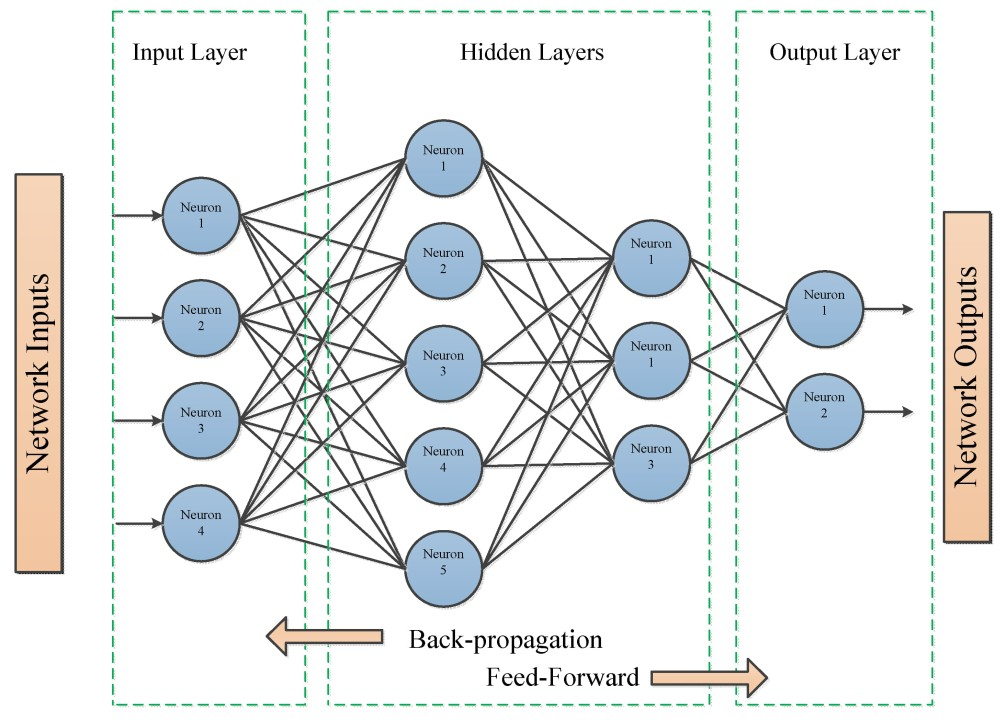
\includegraphics[width=0.7\linewidth]{resources/backpropagation.jpeg}
    \caption{Vzratno razširjanje napake. Vir:~\cite{electronics10212689}}~\label{fig:backprop}
\end{figure}

Od sedaj naprej nas bo samo zanimala evolucija uteži v procesu učenja. Na posameznih slojih bomo opazovali vektorje uteži za vsak nevron, ki jih bomo interpretirali kot točke v visoko dimenzionalnem prostoru. Za vsak sloj $i$ so to  ravno vrstice v matriki uteži $W^{(i)}$. Ker pa si visoko dimenzionalnih prostorov ne moremo predstavljati, se bomo v naslednjem razdelku ukvarjali s tem kako točke preslikati v nižje dimenzionalni prostor s čim manjšo izgubo informacij.
